\documentclass{article}
\usepackage{amsmath}
\usepackage{amsfonts}
\usepackage{amssymb}
\usepackage{enumitem}
\usepackage{tikz}
\usepackage{mathtools}

\usetikzlibrary{arrows}

\title{CSC 226 - Assignment 4 - Theory}
\date{April 2017}
\author{Daniel Frankcom}

\begin{document}
	\pagenumbering{gobble}
	\maketitle
	\setlength{\parindent}{0pt}
	\newcommand{\forceindent}{\leavevmode{\parindent=72pt\indent}}
	\newpage
	\pagenumbering{arabic}
	
	\begin{enumerate}
		\item \quad
		\newline
		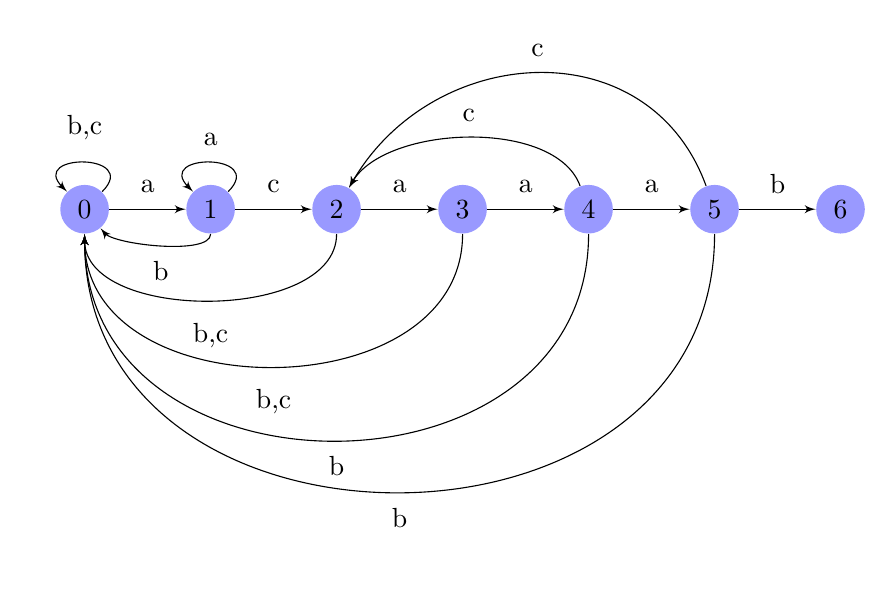
\begin{tikzpicture}
		[scale=.8,auto=left,every node/.style={circle,fill=blue!40}, edge/.style={->,> = latex'}]
		\node (n0) at (0,0)  {0};
		\node (n1) at (2,0)  {1};
		\node (n2) at (4,0)  {2};
		\node (n3) at (6,0)  {3};
		\node (n4) at (8,0)  {4};
		\node (n5) at (10,0)  {5};
		\node (n6) at (12,0)  {6};
		
		\draw[edge] (n0) to node [above, fill=none] {a} (n1);
		\draw[edge] (n1) to node [above, fill=none] {c} (n2);
		\draw[edge] (n2) to node [above, fill=none] {a} (n3);
		\draw[edge] (n3) to node [above, fill=none] {a} (n4);
		\draw[edge] (n4) to node [above, fill=none] {a} (n5);
		\draw[edge] (n5) to node [above, fill=none] {b} (n6);
		
		\draw[edge] (n0) to [out=45,in=135,looseness=4] node [above, fill=none] {b,c} (n0);
		\draw[edge] (n1) to [out=270,in=310,looseness=0.5] node [below, fill=none] {b} (n0);
		\draw[edge] (n1) to [out=45,in=135,looseness=4] node [above, fill=none] {a} (n1);
		\draw[edge] (n2) to [out=270,in=270,looseness=0.9] node [below, fill=none] {b,c} (n0);
		\draw[edge] (n3) to [out=270,in=270,looseness=1.2] node [below, fill=none] {b,c} (n0);
		\draw[edge] (n4) to [out=270,in=270,looseness=1.4] node [below, fill=none] {b} (n0);
		\draw[edge] (n4) to [out=110,in=60,looseness=0.8] node [above, fill=none] {c} (n2);
		\draw[edge] (n5) to [out=270,in=270,looseness=1.4] node [below, fill=none] {b} (n0);
		\draw[edge] (n5) to [out=110,in=60,looseness=1.2] node [above, fill=none] {c} (n2);
		
		\end{tikzpicture}
		
		\item Any example where both the search and pattern strings are entirely made up of one character performs poorly, as the algorithm is not able to skip forward when comparing characters.
		\newline Search string:\hspace{10pt} "AAAAAAAAAAAAAAAA"
		\newline Pattern string:\quad "AA"
		
		\item
		
		\item
		
		\item This problem can be simply reduced to a max flow problem by creating a residual graph where each edge in $G$ is represented as an edge with flow 1. In this manner, when an arbitrary path is chosen during the computation of the max flow, the 1 unit of flow will no longer be available, so we will not choose another path which repeats the same edge.
	\end{enumerate}
\end{document}